% Changing book to article will make the footers match on each page,
% rather than alternate every other.
%
% Note that the article class does not have chapters.
\documentclass[a4paper,9pt,twoside,twocolumn,openany]{book}

\usepackage[utf8]{inputenc}
\usepackage[OT2, T1]{fontenc}

% Use babel or polyglossia to automatically redefine macros for terms
% Armor Class, Level, etc...
% Default output is in English; captions are located in lib/dndstring-captions.sty.
% If no captions exist for a language, English will be used.
%1. To load a language with babel:
%	\usepackage[<lang>]{babel}
%2. To load a language with polyglossia:
%	\usepackage{polyglossia}
%	\setdefaultlanguage{<lang>}
\usepackage[french]{babel}
%usepackage[italian]{babel}
% For further options (multilanguage documents, hypenations, language environments...)
% please refer to babel/polyglossia's documentation.

\usepackage{lipsum}
\usepackage{listings}
\usepackage{swe}
\usepackage{pdfpages}
\usepackage{tikz}
\usepackage{xcolor} 
\definecolor{ultramarine}{RGB}{56,77,61}

\settoggle{justified}{true}
\justifying 

\lstset{%
  basicstyle=\ttfamily,
  language=[LaTeX]{TeX},
}

% Start document
\begin{document}

\includepdf[pages=1,%
    picturecommand*={%
    \put(30,30){ {\huge \scshape \textbf{ \sffamily\bfseries \color{ultramarine} Journal de Bord - Ibu Bul}} }%
}]{img/Front2.pdf}



% Seconde de couverture

\chapter{Généralités et Crédits}

\section{Maître du jeu}

\paragraph{Pibeto} Empire, Résistance, Rebelles, Animaux, Ambiance, ... \emph{Merci à lui.}

\section{Joueurs}

\paragraph{`Oola `Dira, (BSJ)} Twi’lek de couleur orange, mécano, † en otage.
\paragraph{Wesk-Fen Bok 'iort (Fred)} Botan, † dans un combat
\paragraph{Nyr Ch'iort (Natacha)} Botan, signe distinctif des ailes d’anges, pilote.
\paragraph{Wootang (Nboo)} Wookie médecin et éclaireur
\paragraph{Nopok Atol (Ghe)} Rodien verdâtre de 19 ans, chasseur de primes et sniper, † dans un combat.
\paragraph{Kane Starkiller (Rro)} Humain de 23 ans, 1m98, mercenaire maraudeur très bon au corps à corps.
\paragraph{Kar Lya 'Dren (Yo)} Botan, tech/sliceur
\paragraph{Irys Thri 'iya (Christelle)} Botan, disparue à ce jour
\paragraph{Kalcir Thuk} Chasseuse de primes
\paragraph{Ibu Bul} voyageur (BSJ)

\section{Le vaisseau}
Cargo léger \emph{VCX-100}
\emph{\color{red}\MakeUppercase{\textcyr{надежда}}}

\section{Quelques aides et rappels}

\subsection{Investir}

\begin{dndtable}[p{0.3\columnwidth}X]
  \textbf{Achat}                & \textbf{Description} \\
  Compétence carrière           & 5 * seuil (5, 10, 15, ...) \\
  Compétence hors carrière      & 5 * seuil + 5 (5, 10, 15, ...) \\
  Arbre de spéc.                & 10 xp * nb. tot. specs. \\
  .... si nouvel                & Majoration de 10 xp \\
\end{dndtable}

\section{Symbolique}

\begin{dndtable}[cX]
  \textbf{Dés}                & \textbf{Description} \\
  \boost         & aide, bonus \\
  \setback       & contrainte, malus \\
  \difficulty    & difficulté \\
  \ability       & habilité \\
  \challenge     & challenge \\
  \proficiency   & efficacité \\
\end{dndtable}

\begin{dndtable}[cX]
  \textbf{Symbole}  & \textbf{Description} \\
  \successA & Succès \\
  \failureA & \'Echec \\
  \advantage    & Avantage \\
  \threat       & Menace \\
  \triumph   & Triomphe \\
  \despair   & Fumble \\
\end{dndtable}

\newpage

\tableofcontents

\chapter{Les personnages}

\section{Ibu Bul}

\paragraph{\^Age} Temps humain … 23 ans
\paragraph{Sexe} Masculin
\paragraph{Race} Klatooinien

\begin{wrapfigure}{O}{0.25\textwidth}
    
\includegraphics[width=0.25\textwidth]{img/klatooinien.png}
    \caption{Ibu Bul}
\end{wrapfigure}

Ibu est un vagabond parcourant la galaxie à la recherche de nouveaux frissons de traque. Il associe donc sa recherche de proie à son envie de retrouver les membres de son clan\footnote{Motivation "Les égarés" -Au coeur de l'inconnu - p32)}.

Ce sont ses péripéties aux travers de différentes planètes et contrées que ses aptitudes de prédateur se sont développées, afin de s'infiltrer et progresser dans les différents milieux.

Il ne cherche pas à éliminer ses proies ou ses ennemis, car les proies vivantes sont plus intéressantes pour leur prix.

Cela fait maintenant quelques semaines qu'il a entendu parlé de Cholgana et de sa faune riche en proies de choix, avec en particulier les Nexus. Les informations qu’il a pu glaner l’on conduit à chercher des soit disant survivants de la planète sauvage du côté de la Roue et à s’y équiper d’une arme de grande qualité.

Après quelques péripéties, il a pu convaincre de son sérieux et a été invité à se rendre à bord d’un vaisseau très discret, base d’opération de la société Isotech.

C’est à bord qu'il a rencontré Reom qui lui a confié un fusil de sniper de haute qualité moyennant une dette. Il est depuis en attente d’un moyen de transport fiable vers Cholgana ou tout autre lieu qui le conduiront vers des membres de son clan ou des proies intéressantes.

\section{Une nouvelle équipe}
\subtitle{8 décembre 2019}

Un nouveau départ...

C'est donc avec la volonté de mieux connaître Cholgana que je rejoins ce groupe étrange de combattants. En effet, ils sont suspicieux et préfèrent pour l'instant résoudre une mission en cours. C'est donc sur le trajet vers Botawi\footnote{20 crédits pour le trajet} que nous faisons connaissance. Sur place, nous rejoignons leurs collègues à bord d'un vcx100 (figure~\ref{vcx100}). La mission à laquelle je me joins est de récupérer des clefs dans un bureau de société, dans le diamant noir, très haut building.

\begin{wrapfigure}{I}{0.6\columnwidth}
    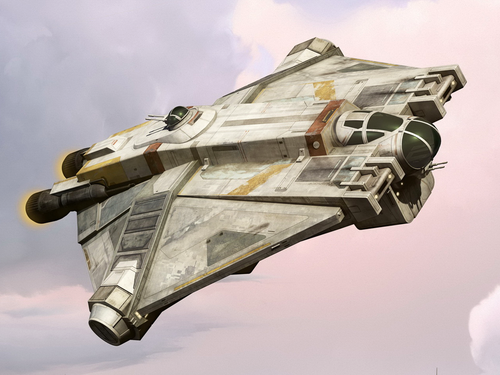
\includegraphics[width=0.6\columnwidth]{img/vcx100.png}
    
    \caption{\MakeUppercase{\textcyr{надежда}}}\label{vcx100}
\end{wrapfigure}


En effet, un certain Sirus s'est volatilisé et il était très proche de Iliat Industries. C'est une société minière, probablement une société écran pour Marson, un fabricant d'armes. Le slicer, dénommé Khar désactive les alarmes de l'étage supérieur en travaux et c'est par ici que nous nous infiltrons. C'est à ce moment que je vois l'humain se servir de ce qui semble un sabre laser. \emph{Il maîtriserait donc la force !}.

Nous arrivons donc à nous emparer des clefs sans faire aucune victimes et nous nous enfuyons en speeder.

Le décryptage des clefs nous informe que Sirus s'appelle en réalité Révan Adara, c'est un démolisseur. Nous demandons plus d'informations, découvrons que le clan Gorensla gère le secteur, c'est un clan de Hutt. OotiSushi, un botan pourrait nous aider à continuer notre investigation sur ce certain Sirus.

\clearevenpage

% Création de la quatrième de couverture
\onecolumn
\Large

\centering

\vfill


\includegraphics[width=1\textwidth]{img/SWEotE}


\vfill

L'histoire de quelques gars et demoiselles à travers l'espace.
\vfill

% End document
\end{document}
